\documentclass{beamer}

% Romanian Language support
\usepackage{ucs}
\usepackage[utf8x]{inputenc}
\PrerenderUnicode{aâîțșĂÎÂȚȘ}
\usepackage[english,romanian]{babel}

\usepackage{hyperref}   % use \url{http://$URL} or \href{http://$URL}{Name}
\usepackage{verbatim}
\usepackage{underscore} % underscores need not be escaped
\usepackage{booktabs}   % nice looking tables
\usepackage{array}      % column size options in tables
\usepackage[normalem]{ulem}       % for striketrough text

\mode<presentation>
%{ \usetheme{Berlin} }

% Disable useless navigation symbols.
\setbeamertemplate{navigation symbols}{}

\title[Despre dezvăț]{Despre dezvăț: Uneori strici ca să construiești}
\institute{InfoEducație 2016 (Gălăciuc, Vrancea)}
\author[Răzvan Deaconescu]{Răzvan Deaconescu \\
razvan.deaconescu@cs.pub.ro}
\date{5 august 2016}

\begin{document}

\frame{\titlepage}

\begin{frame}{În ce direcție merge autobuzul?}
  \begin{figure}
    \centering
    
\includegraphics[width=0.7\textwidth]{img/bus-direction}
  \end{figure}
  \begin{center}
    \scriptsize
    \url{http://www.reatrey.com/wp-content/uploads/2016/02/Screenshot_1-6.jpg}
  \end{center}
\end{frame}

\begin{frame}{Fizz Buzz Test}
  \begin{center}
    \small
    \url{http://c2.com/cgi/wiki?FizzBuzzTest}
  \end{center}
  \scriptsize
  \pause \textit{The Fizz-Buzz test is an interview question designed to help filter out the 99.5\% of programming job candidates who can't seem to program their way out of a wet paper bag. The text of the programming assignment is as follows:} \\
  \vspace{3mm}
  \pause \textit{Write a program that prints the numbers from 1 to 100. But for multiples of three print ``Fizz'' instead of the number and for the multiples of five print ``Buzz''. For numbers which are multiples of both three and five print ``FizzBuzz''.} \\
  \vspace{3mm}
  \pause \textit{I think Fizz-Buzz is ``hard'' for some programmers because (\#1) it doesn't fit into any of the patterns that were given to them in school assignments, and (\#2) it isn't possible to directly and simply represent the necessary tests, without duplication, in just about any commonly-used modern programming language.} \\
\end{frame}

\begin{frame}{Experimentul cu maimuțele}
  \begin{figure}
    \centering
    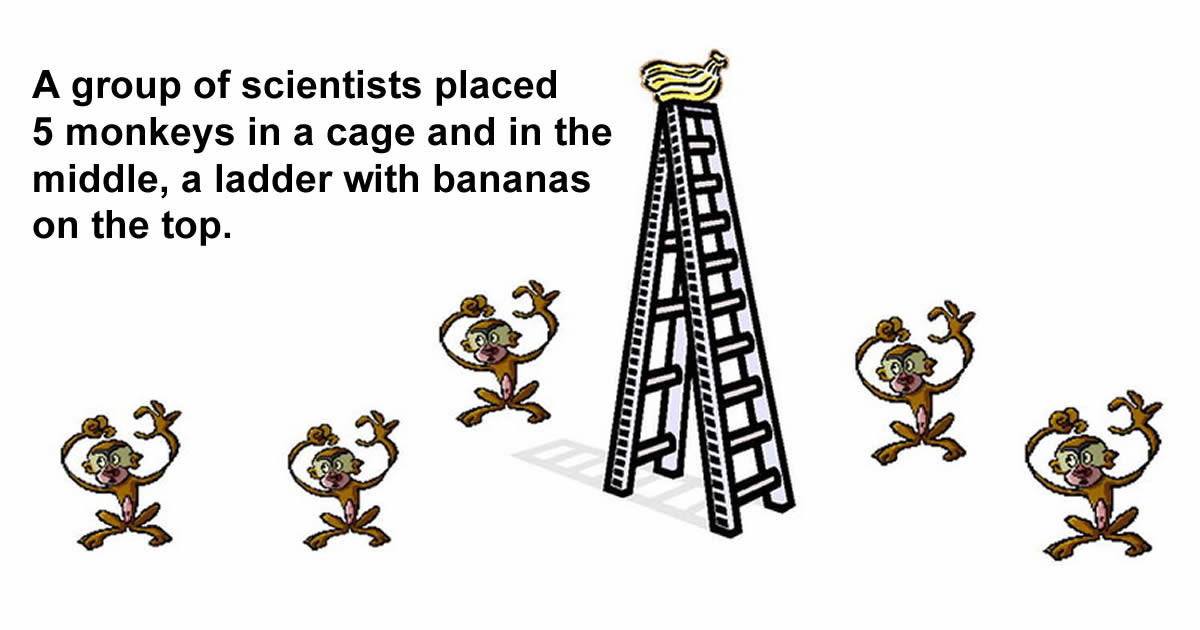
\includegraphics[width=0.8\textwidth]{img/monkey-experiment}
  \end{figure}
  \begin{center}
    \tiny
    \url{http://9gag.com/gag/aA1Z16o/curious-monkey-experiment-are-you-a-blind-follower}
  \end{center}
\end{frame}

\begin{frame}{It's all about the money}
  \begin{itemize}
    \pause \item Ești manager.
    \pause \item Ai nevoie ca echipa pe care o conduci să vină cu soluții creative la o problemă.
    \pause \item Le spui că le acorzi un bonus de 25\% dacă vin astfel de soluții.
  \end{itemize}
  \pause
  \begin{center}
    Dan Pink: The Suprising Truth About What Motivates Us\\
    \vspace{3mm}
    \scriptsize
    \url{http://www.ted.com/talks/dan_pink_on_motivation?language=en}
  \end{center}
\end{frame}

\begin{frame}{Cum învățăm?}
  \begin{itemize}
    \pause \item de la cei din jur
    \pause \item din experiență
    \pause \item din societate
    \pause \item din ce vedem, auzim, ascultăm
    \pause \item din ce citim
    \pause \item de pe Internet
  \end{itemize}
\end{frame}

\begin{frame}{Problema Internet-ului}
  \begin{itemize}
    \pause \item multă informație
    \item informația nu este filtrată
    \pause \item îți dă soluția la problemă, nu cum ajungi la ea
    \pause \item Google/StackOverflow considered harmful
  \end{itemize}
  \pause
  \vspace{1cm}
  \centering
  \textit{Computers are useless. They can only give you answers.}\\
  \vspace{3mm}
  \hfill \textit{Pablo Picasso}
\end{frame}

\begin{frame}{Imperfecțiuni și inabilități}
  \begin{itemize}
    \pause \item informații incomplete
    \pause \item obiceiuri ineficiente
    \pause \item prejudecăți
    \pause \item egocentrism: eu știu (mai bine), eu nu mă înșel (niciodată)
    \pause \item autoritate inadecvată: \textit{It must be true, it's on the Internet.}
    \pause \item presiune socială: așa e bine, așa se întâmplă
    \pause \item (poveste) despre strâmbat
  \end{itemize}
\end{frame}

\begin{frame}{De ce se întâmplă?}
  \begin{itemize}
    \pause \item lene
    \pause \item lipsă de răbdare
    \pause \item neconștientizarea alternativei
    \pause \item influență mare a celor din jur
    \pause \item absența gândirii critice
    \pause \item bias-uri: confirmation bias
    \pause \item instinctul de turmă, ,,compliance''
    \pause \item bulă socială
    \pause \item \url{http://www.throwcase.com/2014/12/21/that-five-monkeys-and-a-banana-story-is-rubbish/}
  \end{itemize}
\end{frame}

\begin{frame}{Luke Skywalker: Too Old}
  \begin{figure}
    \centering
    
\includegraphics[width=0.7\textwidth]{img/yoda-too-old}
  \end{figure}
  \begin{center}
    \scriptsize
    \url{https://memegenerator.net/instance/65152287}
  \end{center}
\end{frame}

\begin{frame}{De ce e rău că se întâmplă?}
  \begin{itemize}
    \pause \item împrăștii dezinformare, cultivi ignoranță
    \pause \item nu îți atingi potențialul, te auto-limitezi
    \pause \item te rigidizezi, nu te adaptezi, te ,,fosilizezi''
    \pause \item lumea este în mișcare rapidă, e dinamică
  \end{itemize}
\end{frame}

\begin{frame}{Cea mai bună întrebare. Cel mai bun răspuns.}
  \centering
  \pause stai în banca ta \\
    \pause vs. \\
  \pause bagă-te în față, dă din coate\\
  \pause
  \vspace{5mm}
  \textit{Courage is what it takes to stand up and speak; courage is also what it takes to sit down and listen.}\\
  \vspace{3mm}
  \hfill \textit{Winston Churchill}\\
  \vspace{5mm}
  \pause Cea mai bună întrebare: \textbf{De ce?} \\
  \pause Cel mai bun răspuns: \textbf{Depinde}
\end{frame}

\begin{frame}{Despre dezvăț}
  \begin{itemize}
    \pause \item renunțat la obiceiuri, comportamente, gânduri, moduri de abordare
    \pause \item alterat obiceiuri, comportamente, gânduri, moduri de abordare
    \pause \item stricat și construit
    \pause \item Pink Floyd: \textit{https://en.wikipedia.org/wiki/The\_Wall}
  \end{itemize}
\end{frame}

\begin{frame}{Exemple și discuție}
  Răzvan
\end{frame}

\begin{frame}{Pași pentru dezvăț}
  \begin{enumerate}
    \pause \item conștientizare
    \pause \item găsit soluție
    \pause \item efort (really really really hard)
    \pause \item reconstruire
    \pause \item menținut flexibilitate
  \end{enumerate}
\end{frame}

\begin{frame}{Cum conștientizăm?}
  \begin{itemize}
    \pause \item introspecție
    \pause \item ,,citim'' în jur
  \end{itemize}
  \pause
  \begin{figure}
    \centering
    
\includegraphics[width=0.4\textwidth]{img/getting-nasty-feedback.jpg}
  \end{figure}
  \begin{itemize}
    \pause \item primirea feedback-ului: Denial, Anger, Withdrawal, Acceptance
    \pause \item oferă, primește, cere, folosește, ia-o de la capăt
  \end{itemize}
\end{frame}

\begin{frame}{Cum construim?}
  \begin{itemize}
    \pause \item acceptarea imperfecțiunilor
    \pause \item puterea de a spune nu știu
    \pause \item puterea de a nu te băga în ce nu ține de tine
    \pause \item conservarea timpului, atenției și energiei
    \pause \item filtarea exteriorului
  \end{itemize}
  \pause
  \vspace{5mm}
  \centering
  \textit{
  Nu vorbi fără să știi \\
  Nu hali mereu ce auzi de la alții, \\
  Nu te da ce nu poți să fii \\
  Sunt vorbe de c***t, le-aud în fiecare zi \\
  }
  \vspace{3mm}
  \hfill \textit{La Familia feat. Uzzi: Vorbe}
\end{frame}

\begin{frame}{Recomandări}
  \begin{itemize}
    \pause \item Gândiți-vă la probleme, nu doar la soluții.
    \pause \item Faceți jocuri de logică, gândire laterală.
    \pause \item Călătoriți și stați printre oameni.
    \pause \item Interacționați cu oameni diferiți.
    \pause \item Jocuri de logică și gândire laterală.
    \pause \item Faceți puzzle-uri.
      \begin{itemize}
        \item Enigma: \tiny{\url{https://www.puzzlemaster.ca/browse/wire/308-cast-enigma-metal}}
      \end{itemize}
  \end{itemize}
  \pause
  \vspace{5mm}
  \centering
  \textit{My mind is my weapon. My brother has his sword, King Robert has his warhammer and I have my mind\ldots{} and a mind needs books as a sword needs a whetstone if it is to keep its edge. That's why I read so much, Jon Snow.}\\
  \vspace{3mm}
  \hfill \textit{Tyrion Lannister}
\end{frame}

\begin{frame}{Recomandări (2)}
  \begin{itemize}
    \pause \item Folosiți mai multe limbaje de programare. Contează problema, nu limbajul.
    \pause \item Învățați programare funcțională.
    \pause \item Folosiți Linux.
    \pause \item Faceți lucrurile și altfel.
  \end{itemize}
\end{frame}

\begin{frame}{Recomandări (3)}
  \begin{itemize}
    \pause \item Meditați, analizați-vă.
    \pause \item Explorați-vă.
    \pause \item Simțiți. Folosiți-vă emoțiile.
    \pause \item Cereți feedback. Acceptați feedback.
    \pause \item Bucurați-vă!
  \end{itemize}
\end{frame}

\begin{frame}{În loc de final}
  \begin{figure}
    \centering
    
\includegraphics[width=0.4\textwidth]{img/michelangelo-ancora-imparo.jpg}
  \end{figure}
  \begin{center}
    \tiny
    \url{http://learnteachserve.org/wp-content/uploads/2014/04/michelangelo_ancora-imparo.jpg}
  \end{center}
\end{frame}

\end{document}
